\documentclass[11pt,a4paper]{article}

\usepackage[utf8]{inputenc}
\usepackage[spanish,es-nodecimaldot]{babel}
\usepackage[T1]{fontenc}
\usepackage{lmodern}
\usepackage{geometry}
\geometry{top=2.5cm, bottom=2.5cm, left=2.5cm, right=2.5cm}

\usepackage{amsmath,amssymb}
\usepackage{graphicx}
\usepackage{booktabs}
\usepackage{float}
\usepackage{hyperref}
\hypersetup{colorlinks=true, linkcolor=black, urlcolor=blue}

\setlength{\parindent}{0pt}
\setlength{\parskip}{6pt}

\title{
    \vspace{-1.2cm}
    \textbf{Sistemas de Control}\\
    \large Trabajo de Laboratorio Integrador: Modelado y Simulación
}
\author{Tomás Gómez Pizarro \quad\and\quad Mikael Rodríguez}
\date{Octubre 2026}

\begin{document}

\maketitle

\section*{Parte A. Modelado y análisis}

\begin{figure}[H]
    \centering
    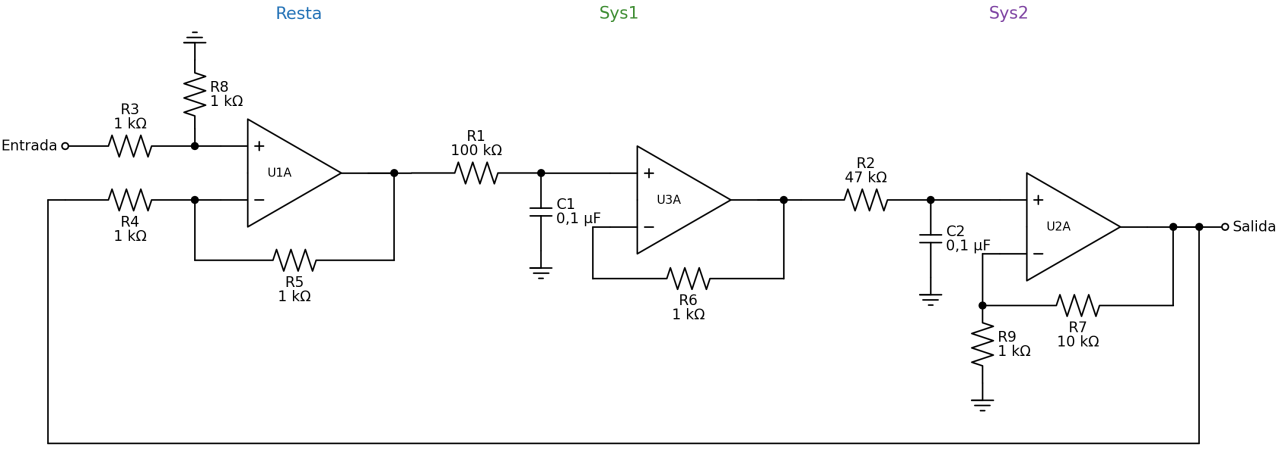
\includegraphics[width=0.85\textwidth]{figuras/figura_1.png}
    \caption{Planta a controlar (alimentación de los operacionales: $\pm 10\text{ V}$).}
    \label{fig:circuito}
\end{figure}

\begin{figure}[H]
    \centering
    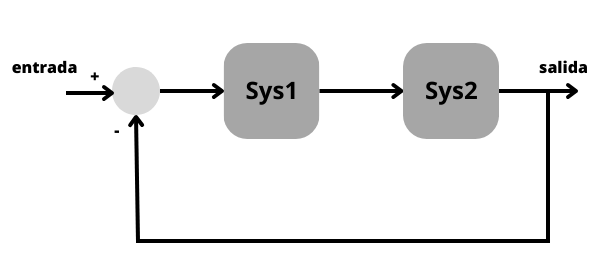
\includegraphics[width=0.5\textwidth]{figuras/figura_2.png}
    \caption{Diagrama de bloques de la planta a controlar.}
    \label{fig:bloques}
\end{figure}

\section{Modelado}

\subsection{Funciones de transferencia por bloques (Fig. 2)}
Considerando amplificadores operacionales ideales en zona lineal ($I_+ = I_- = 0$ y $V_+ = V_-$):

\paragraph{Bloque Resta ($U_{1A}$):}
En el terminal no inversor tenemos un divisor resistivo entre $R_3$ y $R_8$ ($R_3 = R_8 = 1\text{ k}\Omega$):
\begin{equation}
    V_+ = V_{\text{Entrada}} \frac{R_8}{R_3 + R_8} = \frac{1}{2} V_{\text{Entrada}}
\end{equation}
En el nodo inversor, planteando corrientes con $R_4 = R_5 = 1\text{ k}\Omega$:
\begin{equation}
    \frac{V_{\text{Salida}} - V_-}{R_4} + \frac{V_{\text{resta}} - V_-}{R_5} = 0 \implies V_- = \frac{V_{\text{Salida}} + V_{\text{resta}}}{2}
\end{equation}
Igualando $V_+ = V_-$ resulta:
\begin{equation}
    V_{\text{resta}}(s) = V_{\text{Entrada}}(s) - V_{\text{Salida}}(s)
\end{equation}
Por lo tanto, la etapa con $U_{1A}$ implementa el restador unitario de entrada del lazo.

\paragraph{Bloque $\text{Sys}_1$ ($R_1$, $C_1$ y $U_{3A}$):}
La red $R_1 C_1$ forma un divisor de impedancias a la entrada no inversora de $U_{3A}$. Como $I_+ = 0$:
\begin{equation}
    V_{+,U3A}(s) = \frac{\frac{1}{sC_1}}{R_1 + \frac{1}{sC_1}} V_{\text{resta}}(s) = \frac{1}{R_1 C_1 s + 1} V_{\text{resta}}(s)
\end{equation}
El operacional $U_{3A}$ está conectado como seguidor de tensión ($V_{\text{out},U3A} = V_{+,U3A}$), por lo que con $R_1 = 100\text{ k}\Omega$ y $C_1 = 0,1\,\mu\text{F}$ ($\tau_1 = R_1 C_1 = 0,01\text{ s}$):
\begin{equation}
    \text{Sys}_1(s) = \frac{1}{R_1 C_1 s + 1} = \frac{1}{0,01 s + 1}
\end{equation}

\paragraph{Bloque $\text{Sys}_2$ ($R_2$, $C_2$ y $U_{2A}$):}
De manera análoga, la red $R_2 C_2$ en la entrada no inversora de $U_{2A}$ cumple:
\begin{equation}
    V_{+,U2A}(s) = \frac{1}{R_2 C_2 s + 1} V_{\text{out},U3A}(s)
\end{equation}
El operacional $U_{2A}$ está en configuración no inversora con ganancia $k = 1 + \frac{R_7}{R_9}$. Con $R_2 = 47\text{ k}\Omega$, $C_2 = 0,1\,\mu\text{F}$ ($\tau_2 = R_2 C_2 = 0,0047\text{ s}$) y $k = 1 + \frac{10\text{ k}\Omega}{1\text{ k}\Omega} = 11$:
\begin{equation}
    \text{Sys}_2(s) = \frac{k}{R_2 C_2 s + 1} = \frac{k}{0,0047 s + 1}
\end{equation}
Como el seguidor $U_{3A}$ desacopla ambas etapas, el camino directo es el producto $\text{Sys}_1(s) \cdot \text{Sys}_2(s)$ y el circuito queda representado por el diagrama de bloques de la Fig. \ref{fig:bloques}.

\subsection{Función de transferencia en lazo cerrado $\text{Sys}_f(s)$}
Para el lazo con realimentación negativa unitaria, siendo $G(s) = \text{Sys}_1(s)\text{Sys}_2(s)$:
\begin{equation}
    \text{Sys}_f(s) = \frac{\text{Salida}(s)}{\text{Entrada}(s)} = \frac{G(s)}{1 + G(s)} = \frac{k}{(\tau_1 s + 1)(\tau_2 s + 1) + k}
\end{equation}
Desarrollando el denominador y dividiendo por $\tau_1 \tau_2$:
\begin{equation}
    \text{Sys}_f(s) = \frac{\dfrac{k}{\tau_1 \tau_2}}{s^2 + \left(\dfrac{1}{\tau_1} + \dfrac{1}{\tau_2}\right)s + \dfrac{1 + k}{\tau_1 \tau_2}}
\end{equation}
Reemplazando $\tau_1 = 0,01\text{ s}$, $\tau_2 = 0,0047\text{ s}$ y $k = 11$:
\begin{equation}
    \text{Sys}_f(s) = \frac{234042,55}{s^2 + 312,77\,s + 255319,15}
\end{equation}

\subsection{Parámetros $\omega_n$ y $\xi$, e influencia de $k$}
Comparando el denominador con la forma canónica $s^2 + 2\xi\omega_n s + \omega_n^2$:
\begin{align}
    \omega_n &= \sqrt{\frac{1+k}{\tau_1 \tau_2}} = \sqrt{255319,15} \approx 505,29\text{ rad/s} \\
    \xi &= \frac{1/\tau_1 + 1/\tau_2}{2\omega_n} = \frac{312,77}{2 \cdot 505,29} \approx 0,3095
\end{align}
\textbf{Influencia de $k$:} Al aumentar $k$, la frecuencia natural $\omega_n$ aumenta ($\propto \sqrt{1+k}$), haciendo más rápida la respuesta inicial, mientras que el amortiguamiento $\xi$ disminuye ($\propto 1/\sqrt{1+k}$), provocando mayores oscilaciones y un mayor sobrepaso ($PO$). Sin embargo, el producto $\xi\omega_n = \frac{1}{2}\left(\frac{1}{\tau_1} + \frac{1}{\tau_2}\right) = 156,38\text{ s}^{-1}$ (parte real de los polos de lazo cerrado) no depende de $k$, por lo que el tiempo de establecimiento $T_s \approx \frac{4}{\xi\omega_n}$ se mantiene prácticamente constante. Además, un mayor $k$ acerca la ganancia estacionaria $\frac{k}{1+k}$ a $1$, reduciendo el error permanente.

\subsection{Función de $R_6$ y del seguidor $U_{3A}$}
\begin{itemize}
    \item \textbf{Resistencia $R_6$:} En un circuito real se coloca para igualar la resistencia vista por ambas entradas del operacional y compensar las pequeñas corrientes de entrada del dispositivo. En el modelo ideal, como no ingresa corriente al terminal inversor ($I_- = 0$), no hay caída de tensión en $R_6$ ($\Delta V_{R_6} = 0$) y equivale a un cable directo, razón por la cual no aparece en la función de transferencia.
    \item \textbf{Seguidor $U_{3A}$ y su eliminación:} Gracias a su alta impedancia de entrada, aísla ambas etapas sin tomar corriente de $C_1$, permitiendo obtener la planta simplemente multiplicando los bloques individuales $\text{Sys}_1(s) \cdot \text{Sys}_2(s)$. Si se eliminara $U_{3A}$ conectando $R_2$ directamente sobre $C_1$, la segunda etapa $RC$ cargaría a la primera (derivando corriente de $C_1$ hacia $R_2$) y ya no podrían modelarse como dos bloques independientes en cascada, apareciendo un término de acoplamiento $R_1 C_2 s$ en el denominador:
    \begin{equation}
        G_{\text{sin seguidor}}(s) = \frac{k}{\tau_1 \tau_2 s^2 + (\tau_1 + \tau_2 + R_1 C_2)s + 1}
    \end{equation}
\end{itemize}

\section{Respuesta al escalón de $\text{Sys}_f$ ($k = 11$)}
Como el sistema es subamortiguado ($\xi = 0,3095 < 1$), su frecuencia amortiguada es $\omega_d = \omega_n\sqrt{1 - \xi^2} \approx 480,48\text{ rad/s}$ y el ángulo de fase es $\beta = \arccos(\xi) \approx 1,256\text{ rad}$. Ante una entrada en escalón unitario ($1\text{ V}$), la respuesta temporal analítica es:
\begin{equation}
    y(t) = y(\infty)\left[1 - \frac{e^{-\xi\omega_n t}}{\sqrt{1 - \xi^2}}\sin(\omega_d t + \beta)\right] = 0,9167\left[1 - 1,0516\,e^{-156,38\,t}\sin(480,48\,t + 1,256)\right]\text{ V}
\end{equation}
Los parámetros principales de desempeño son:
\begin{itemize}
    \item \textbf{Valor en estado estacionario:}
    \begin{equation}
        y(\infty) = \lim_{s \to 0} \text{Sys}_f(s) = \frac{k}{1+k} = \frac{11}{12} \approx 0,9167\text{ V}
    \end{equation}
    \item \textbf{Sobrepaso porcentual ($PO$):}
    \begin{equation}
        PO = 100 \cdot e^{-\frac{\pi\xi}{\sqrt{1-\xi^2}}} \approx 35,97\% \quad \left(y_{\max} = y(\infty)(1 + PO/100) \approx 1,246\text{ V}\right)
    \end{equation}
    \item \textbf{Tiempo de pico ($T_p$):}
    \begin{equation}
        T_p = \frac{\pi}{\omega_d} = \frac{\pi}{480,48} \approx 6,54\text{ ms}
    \end{equation}
    \item \textbf{Tiempo de establecimiento ($T_s$, criterio del $2\%$):}
    \begin{equation}
        T_s \approx \frac{4}{\xi\omega_n} = \frac{4}{156,38} \approx 25,58\text{ ms}
    \end{equation}
    \item \textbf{Tiempo de subida ($t_r$, criterio del $10\%$ al $90\%$):}
    \begin{equation}
        t_r \approx \frac{2,16\,\xi + 0,6}{\omega_n} = \frac{2,16 \cdot 0,3095 + 0,6}{505,29} \approx 2,51\text{ ms} \quad (\text{valor exacto } 10\%\text{--}90\%\text{: } 2,57\text{ ms})
    \end{equation}
\end{itemize}

\paragraph{Verificación por simulación en MATLAB:}
A partir de la simulación temporal del modelo en MATLAB ante un escalón de $1\text{ V}$, se obtienen los siguientes parámetros de respuesta:
\begin{itemize}
    \item \textbf{Valor final:} $y(\infty) = 0,9167\text{ V}$ (coincidencia exacta con el valor analítico $11/12\text{ V}$).
    \item \textbf{Sobrepaso porcentual:} $PO = 35,97\%$ (coincide exactamente con el valor teórico analítico).
    \item \textbf{Tiempo de pico:} $T_p = 6,50\text{ ms}$ (en excelente concordancia con los $6,54\text{ ms}$ teóricos).
    \item \textbf{Tiempo de establecimiento ($2\%$):} $T_s = 22,23\text{ ms}$ (instante en que la curva entra y se mantiene en la banda del $\pm 2\%$, frente a la cota teórica conservativa de envolvente $4/(\xi\omega_n) = 25,58\text{ ms}$).
    \item \textbf{Tiempo de subida ($10\%$--$90\%$):} $t_r = 2,57\text{ ms}$ (concordante con la aproximación analítica de $2,51\text{ ms}$).
\end{itemize}

\section{Error en estado estacionario}
La transferencia entre la referencia y el error $E(s) = \text{Entrada}(s) - \text{Salida}(s)$ es:
\begin{equation}
    E(s) = \frac{1}{1 + G(s)} R(s), \qquad G(s) = \frac{k}{(0,01 s + 1)(0,0047 s + 1)}
\end{equation}
Como $G(s)$ no posee polos en el origen ($N = 0$), el sistema es de \textbf{Tipo 0}. Aplicando el Teorema del Valor Final ($e_{ss} = \lim_{s \to 0} s E(s)$):

\begin{itemize}
    \item \textbf{Entrada en escalón unitario ($R(s) = 1/s$):}
    \begin{equation}
        K_p = \lim_{s \to 0} G(s) = k = 11 \implies e_{ss,\text{escalón}} = \frac{1}{1 + K_p} = \frac{1}{1 + k} = \frac{1}{12} \approx 0,0833\text{ V}
    \end{equation}
    \item \textbf{Entrada en rampa unitaria ($R(s) = 1/s^2$):}
    \begin{equation}
        K_v = \lim_{s \to 0} s G(s) = 0 \implies e_{ss,\text{rampa}} = \frac{1}{K_v} = \infty
    \end{equation}
    Al no tener un integrador en lazo abierto, el sistema no puede seguir una entrada en rampa y el error crece indefinidamente con el tiempo.
\end{itemize}

\paragraph{Comprobación por simulación en MATLAB:}
\begin{itemize}
    \item \textbf{Escalón unitario:} Simulando la respuesta temporal de la señal de error en MATLAB, el valor final en régimen permanente converge a $e_{ss,\text{sim}} = 0,0833\text{ V} = 1/12\text{ V}$, coincidiendo exactamente con el cálculo teórico.
    \item \textbf{Rampa unitaria ($r(t) = t$):} Al simular la respuesta del sistema frente a una entrada en rampa unitaria, se evalúa la evolución temporal del error $e(t) = r(t) - y(t)$. Como el sistema es de Tipo 0, la salida sigue a la rampa con una ganancia inferior a la unidad ($\frac{k}{1+k} = \frac{11}{12}\text{ V/s}$), por lo que el error crece linealmente de forma indefinida a una tasa de $\left(1 - \frac{11}{12}\right) = \frac{1}{12}\text{ V/s} \approx 0,0833\text{ V/s}$. La simulación confirma que en $t = 1\text{ s}$ el error es de $0,0833\text{ V}$, en $t = 5\text{ s}$ asciende a $0,4167\text{ V}$ y en $t = 10\text{ s}$ alcanza $0,8333\text{ V}$, comprobando numéricamente que el error en régimen permanente diverge a infinito ($e_{ss} \to \infty$).
\end{itemize}

\section{Respuesta para distintos valores de $k$ (serie E24)}
Para realizar la ganancia $k = 1 + \frac{R_7}{R_9}$ con resistencias comerciales de la serie E24 en el rango de $1\text{ k}\Omega$ a $100\text{ k}\Omega$, fijamos $R_9 = 1\text{ k}\Omega$ y calculamos $R_7 = (k - 1)R_9$, admitiéndose también resistencias de valor cero e infinito según la consigna:
\begin{itemize}
    \item \textbf{$k = 1$:} Se reemplaza $R_7$ por un cortocircuito ($R_7 = 0\,\Omega$) y se desconecta $R_9$ ($R_9 \to \infty$), quedando $U_{2A}$ como seguidor de tensión con $k_{\text{ef}} = 1$.
    \item \textbf{$k = 3,2$:} $R_7 = 2,2\text{ k}\Omega$ y $R_9 = 1\text{ k}\Omega \implies k_{\text{ef}} = 1 + \frac{2,2}{1} = 3,2$.
    \item \textbf{$k = 5,7$:} $R_7 = 4,7\text{ k}\Omega$ y $R_9 = 1\text{ k}\Omega \implies k_{\text{ef}} = 1 + \frac{4,7}{1} = 5,7$.
    \item \textbf{$k = 34$:} $R_7 = 33\text{ k}\Omega$ y $R_9 = 1\text{ k}\Omega \implies k_{\text{ef}} = 1 + \frac{33}{1} = 34$.
\end{itemize}
Como $2,2$, $4,7$ y $33$ son valores exactos de la serie E24, en los cuatro casos el $k$ efectivo coincide exactamente con el valor pedido (error relativo del $0\%$). En la Tabla \ref{tab:punto4} se resumen los parámetros del sistema calculados en MATLAB para cada valor de $k$, en plena concordancia con las expresiones analíticas de los puntos anteriores.

\begin{table}[H]
    \centering
    \begin{tabular}{c c c c c c c c c}
        \toprule
        \textbf{$k$} & \textbf{$R_7 / R_9$} & \textbf{$\omega_n$ [rad/s]} & \textbf{$\xi$} & \textbf{PO [\%]} & \textbf{$T_p$ [s]} & \textbf{$T_s$ [s]} & \textbf{$y(\infty)$} & \textbf{$e_{ss}$} \\
        \midrule
        $1$ & $0\,\Omega$ / $\infty$ & $206,28$ & $0,7581$ & $2,59$ & $0,0234$ & $0,0256$ & $0,5000$ & $0,5000$ \\
        $3,2$ & $2,2\text{ k}\Omega\,/\,1\text{ k}\Omega$ & $298,93$ & $0,5231$ & $14,54$ & $0,0123$ & $0,0256$ & $0,7619$ & $0,2381$ \\
        $5,7$ & $4,7\text{ k}\Omega\,/\,1\text{ k}\Omega$ & $377,56$ & $0,4142$ & $23,94$ & $0,0091$ & $0,0256$ & $0,8507$ & $0,1493$ \\
        $34$ & $33\text{ k}\Omega\,/\,1\text{ k}\Omega$ & $862,95$ & $0,1812$ & $56,05$ & $0,0037$ & $0,0256$ & $0,9714$ & $0,0286$ \\
        \bottomrule
    \end{tabular}
    \caption{Parámetros teóricos de la respuesta al escalón para los cuatro valores de $k$.}
    \label{tab:punto4}
\end{table}

\section*{Parte B. Verificación por simulación circuital}

\section{Circuito con op-amps ideales}

\subsection{Implementación en Simscape}
Se armó el circuito completo de la Fig. \ref{fig:circuito} en Simscape utilizando resistores, capacitores inicialmente descargados ($0\text{ V}$) y amplificadores operacionales ideales para $U_{1A}$, $U_{3A}$ y $U_{2A}$, aplicando un escalón de entrada de $1\text{ V}$ durante $50\text{ ms}$.

\subsection{Comparación de la salida con $\text{Sys}_f(s)$ ($k = 11$)}
En la Fig. \ref{fig:punto5b} se superpone la tensión de salida obtenida en Simscape con la respuesta teórica al escalón de $\text{Sys}_f(s)$.

\begin{figure}[H]
    \centering
    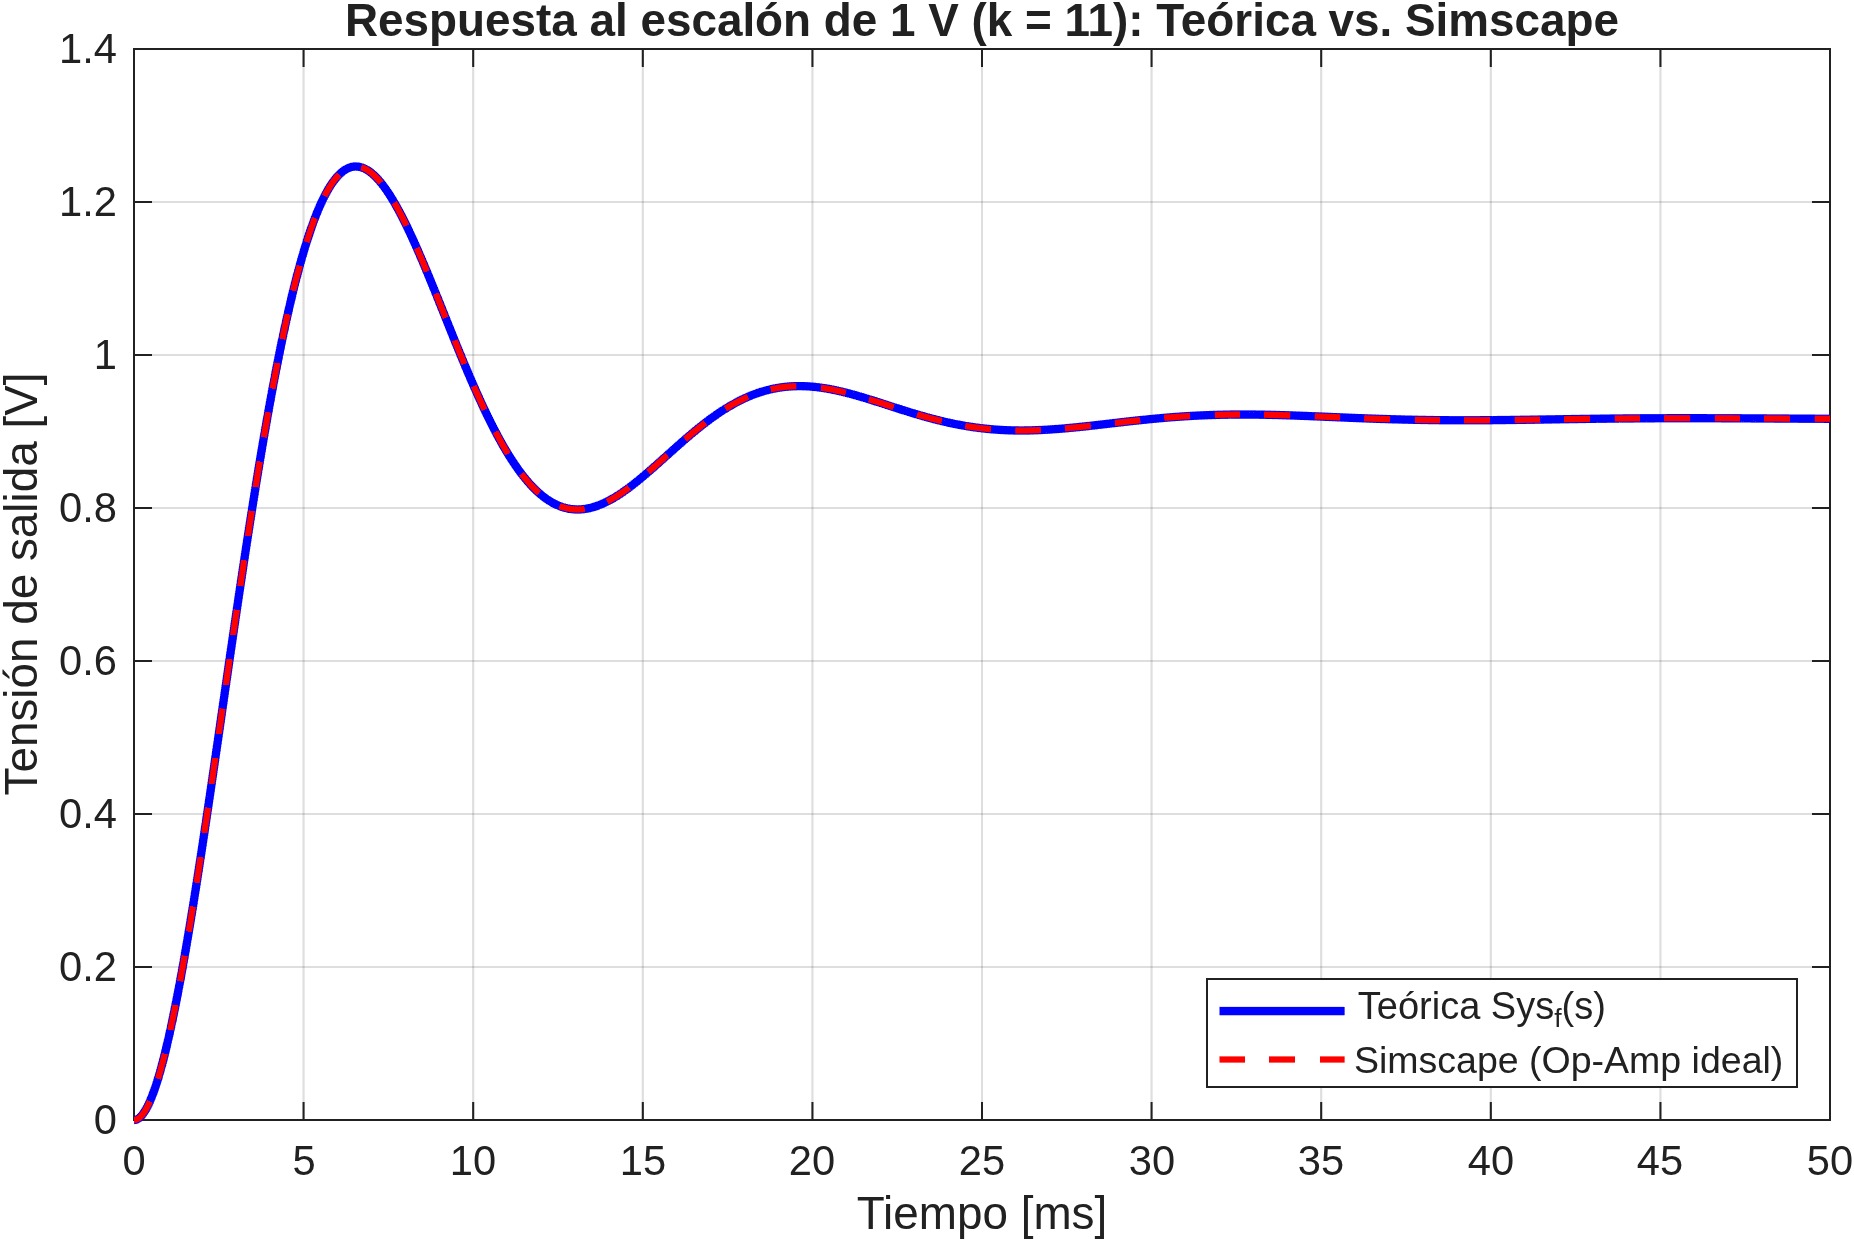
\includegraphics[width=0.78\textwidth]{figuras/punto5b_k11.png}
    \caption{Respuesta al escalón de $1\text{ V}$ para $k = 11$: función de transferencia teórica $\text{Sys}_f(s)$ vs. circuito en Simscape con op-amps ideales.}
    \label{fig:punto5b}
\end{figure}

El error máximo absoluto entre ambas curvas en todo el intervalo de simulación es:
\begin{equation}
    e_{\max} = \max_{t \in [0,\,50\text{ ms}]} \left|y_{\text{teor}}(t) - y_{\text{sim}}(t)\right| = 1,69 \times 10^{-6}\text{ V}
\end{equation}
Ambas respuestas coinciden porque tanto la deducción analítica de $\text{Sys}_f(s)$ como el modelo de op-amp ideal de Simscape asumen corriente de entrada nula ($I_+ = I_- = 0$), ganancia de lazo abierto infinita ($V_+ = V_-$) y ausencia de saturación, de modo que el seguidor $U_{3A}$ aísla las dos etapas $RC$. La mínima diferencia de $1,69\,\mu\text{V}$ se debe únicamente a la tolerancia numérica del simulador.

\subsection{Señal de error $e(t)$ a la salida de $U_{1A}$ ($k = 11$)}
La tensión a la salida del restador $U_{1A}$ corresponde a la señal de error $E(s) = \text{Entrada}(s) - \text{Salida}(s)$. Sabiendo que $\text{Salida}(s) = G(s)E(s)$ con $G(s) = \text{Sys}_1(s)\text{Sys}_2(s)$, la función de transferencia entre la referencia y el error es:
\begin{equation}
    \text{Sys}_e(s) = \frac{E(s)}{\text{Entrada}(s)} = \frac{1}{1 + G(s)} = \frac{(\tau_1 s + 1)(\tau_2 s + 1)}{(\tau_1 s + 1)(\tau_2 s + 1) + k}
\end{equation}
Reemplazando $\tau_1 = 0,01\text{ s}$, $\tau_2 = 0,0047\text{ s}$ y $k = 11$:
\begin{equation}
    \text{Sys}_e(s) = \frac{4,7 \times 10^{-5}\,s^2 + 0,0147\,s + 1}{4,7 \times 10^{-5}\,s^2 + 0,0147\,s + 12} = \frac{s^2 + 312,77\,s + 21276,60}{s^2 + 312,77\,s + 255319,15}
\end{equation}

En la Fig. \ref{fig:punto5c} se superpone la respuesta teórica al escalón de $\text{Sys}_e(s)$ con la tensión medida a la salida de $U_{1A}$ en Simscape.

\begin{figure}[H]
    \centering
    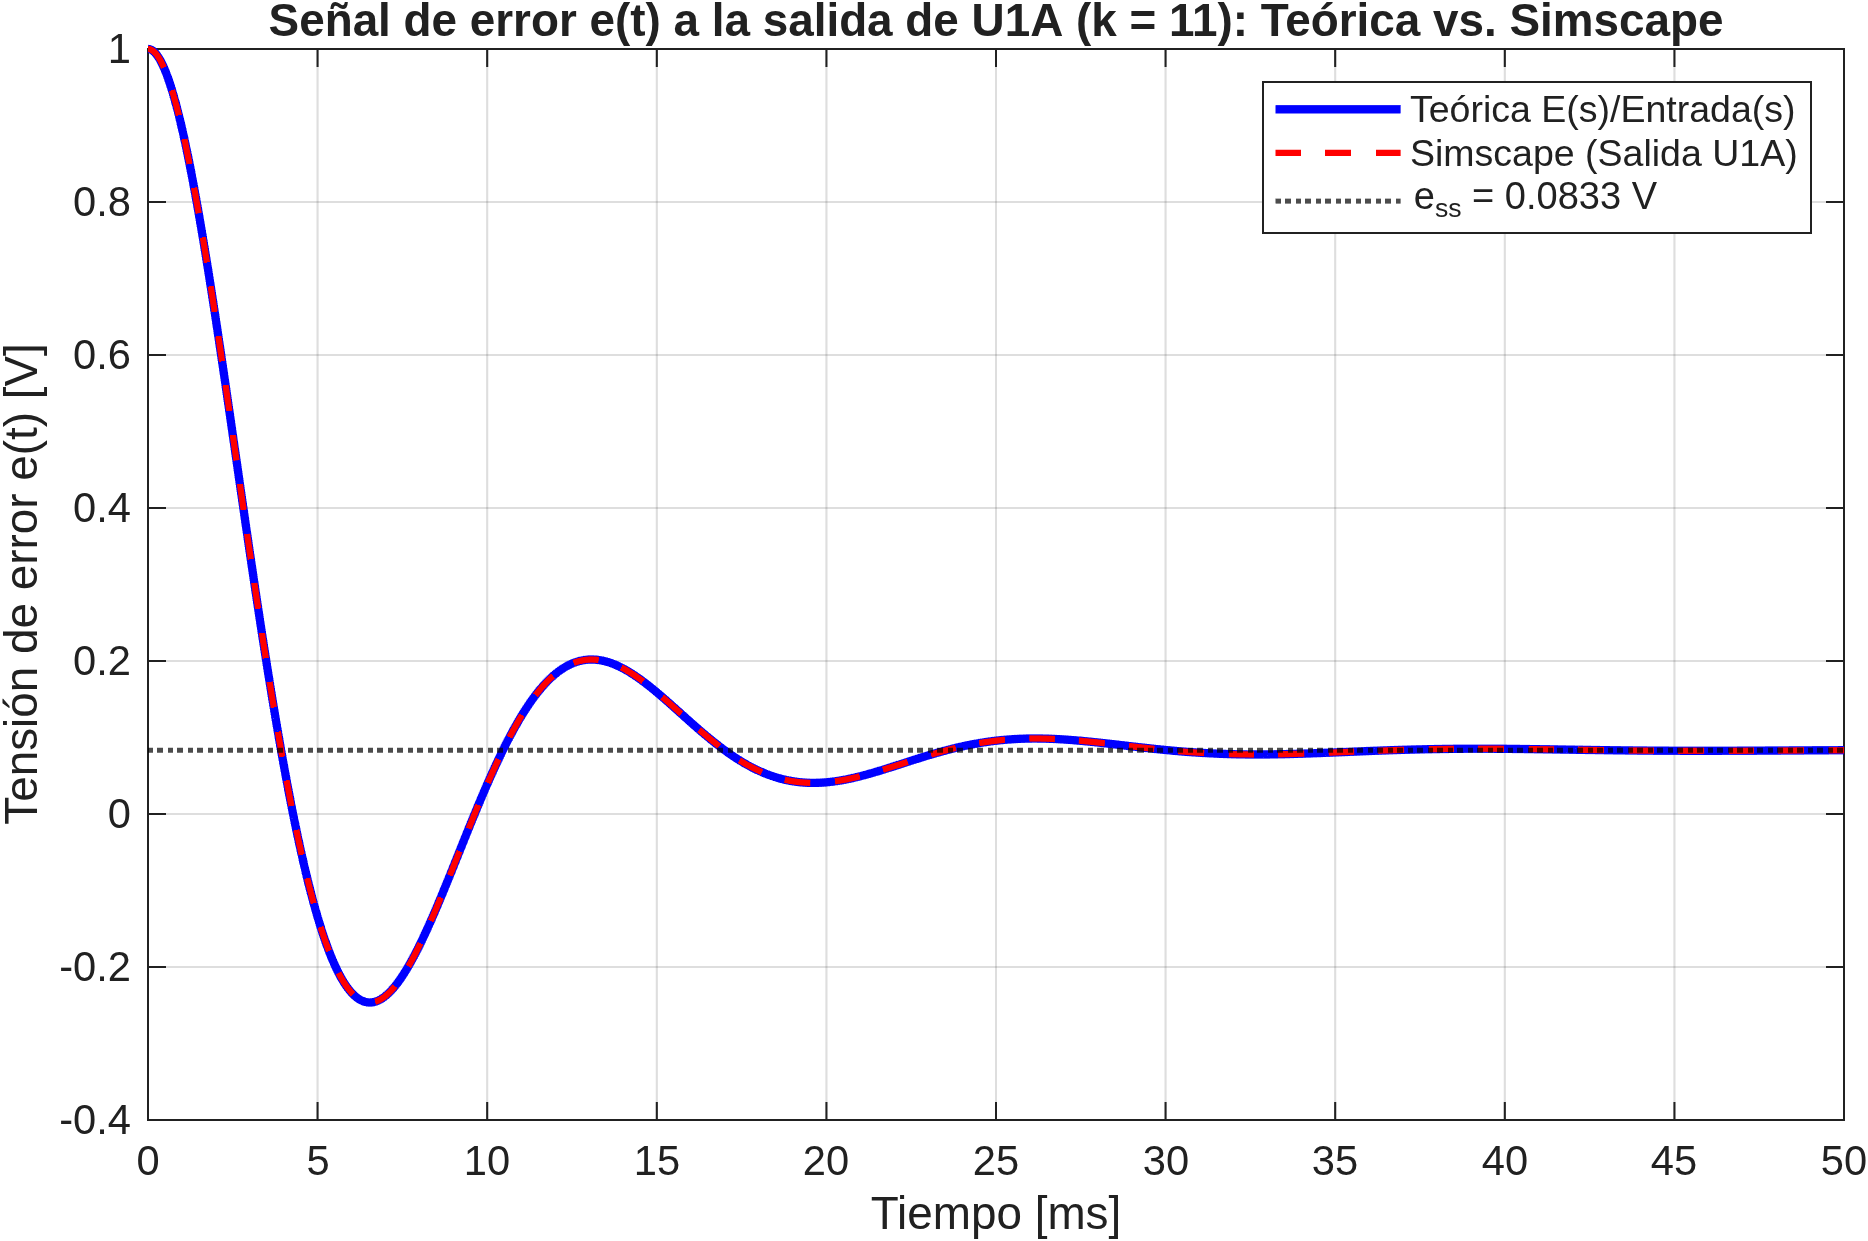
\includegraphics[width=0.78\textwidth]{figuras/punto5c_error_k11.png}
    \caption{Señal de error $e(t)$ a la salida de $U_{1A}$ para un escalón de $1\text{ V}$ ($k = 11$): transferencia teórica $E(s)/\text{Entrada}(s)$ vs. Simscape.}
    \label{fig:punto5c}
\end{figure}

En $t = 0^+$, al estar descargados los capacitores ($y(0^+) = 0\text{ V}$), el error parte de $e(0^+) = 1\text{ V}$. Cuando la salida alcanza su pico máximo de $1,246\text{ V}$ en $T_p \approx 6,54\text{ ms}$, el error toma su valor mínimo negativo ($1 - 1,246 = -0,246\text{ V}$). Finalmente, en régimen permanente la tensión a la salida de $U_{1A}$ converge a:
\begin{equation}
    e_{\text{sim}}(\infty) = 0,0833\text{ V} = \frac{1}{12}\text{ V}
\end{equation}
coincidiendo con el error en estado estacionario $e_{ss} = \frac{1}{1+k}$ calculado en el Punto 3.

\subsection{Comparación para los cuatro valores de $k$ del Punto 4}
Se repitió la simulación en Simscape para $k \in \{1;\, 3,2;\, 5,7;\, 34\}$ fijando $R_9 = 1\text{ k}\Omega$ y empleando los valores comerciales $R_7 \in \{0\,\Omega;\, 2,2\text{ k}\Omega;\, 4,7\text{ k}\Omega;\, 33\text{ k}\Omega\}$. En la Fig. \ref{fig:punto5d} se superponen las respuestas teóricas y simuladas para los cuatro casos, y en la Tabla \ref{tab:punto5d} se comparan los parámetros teóricos frente a los medidos sobre las curvas de Simscape.

\begin{figure}[H]
    \centering
    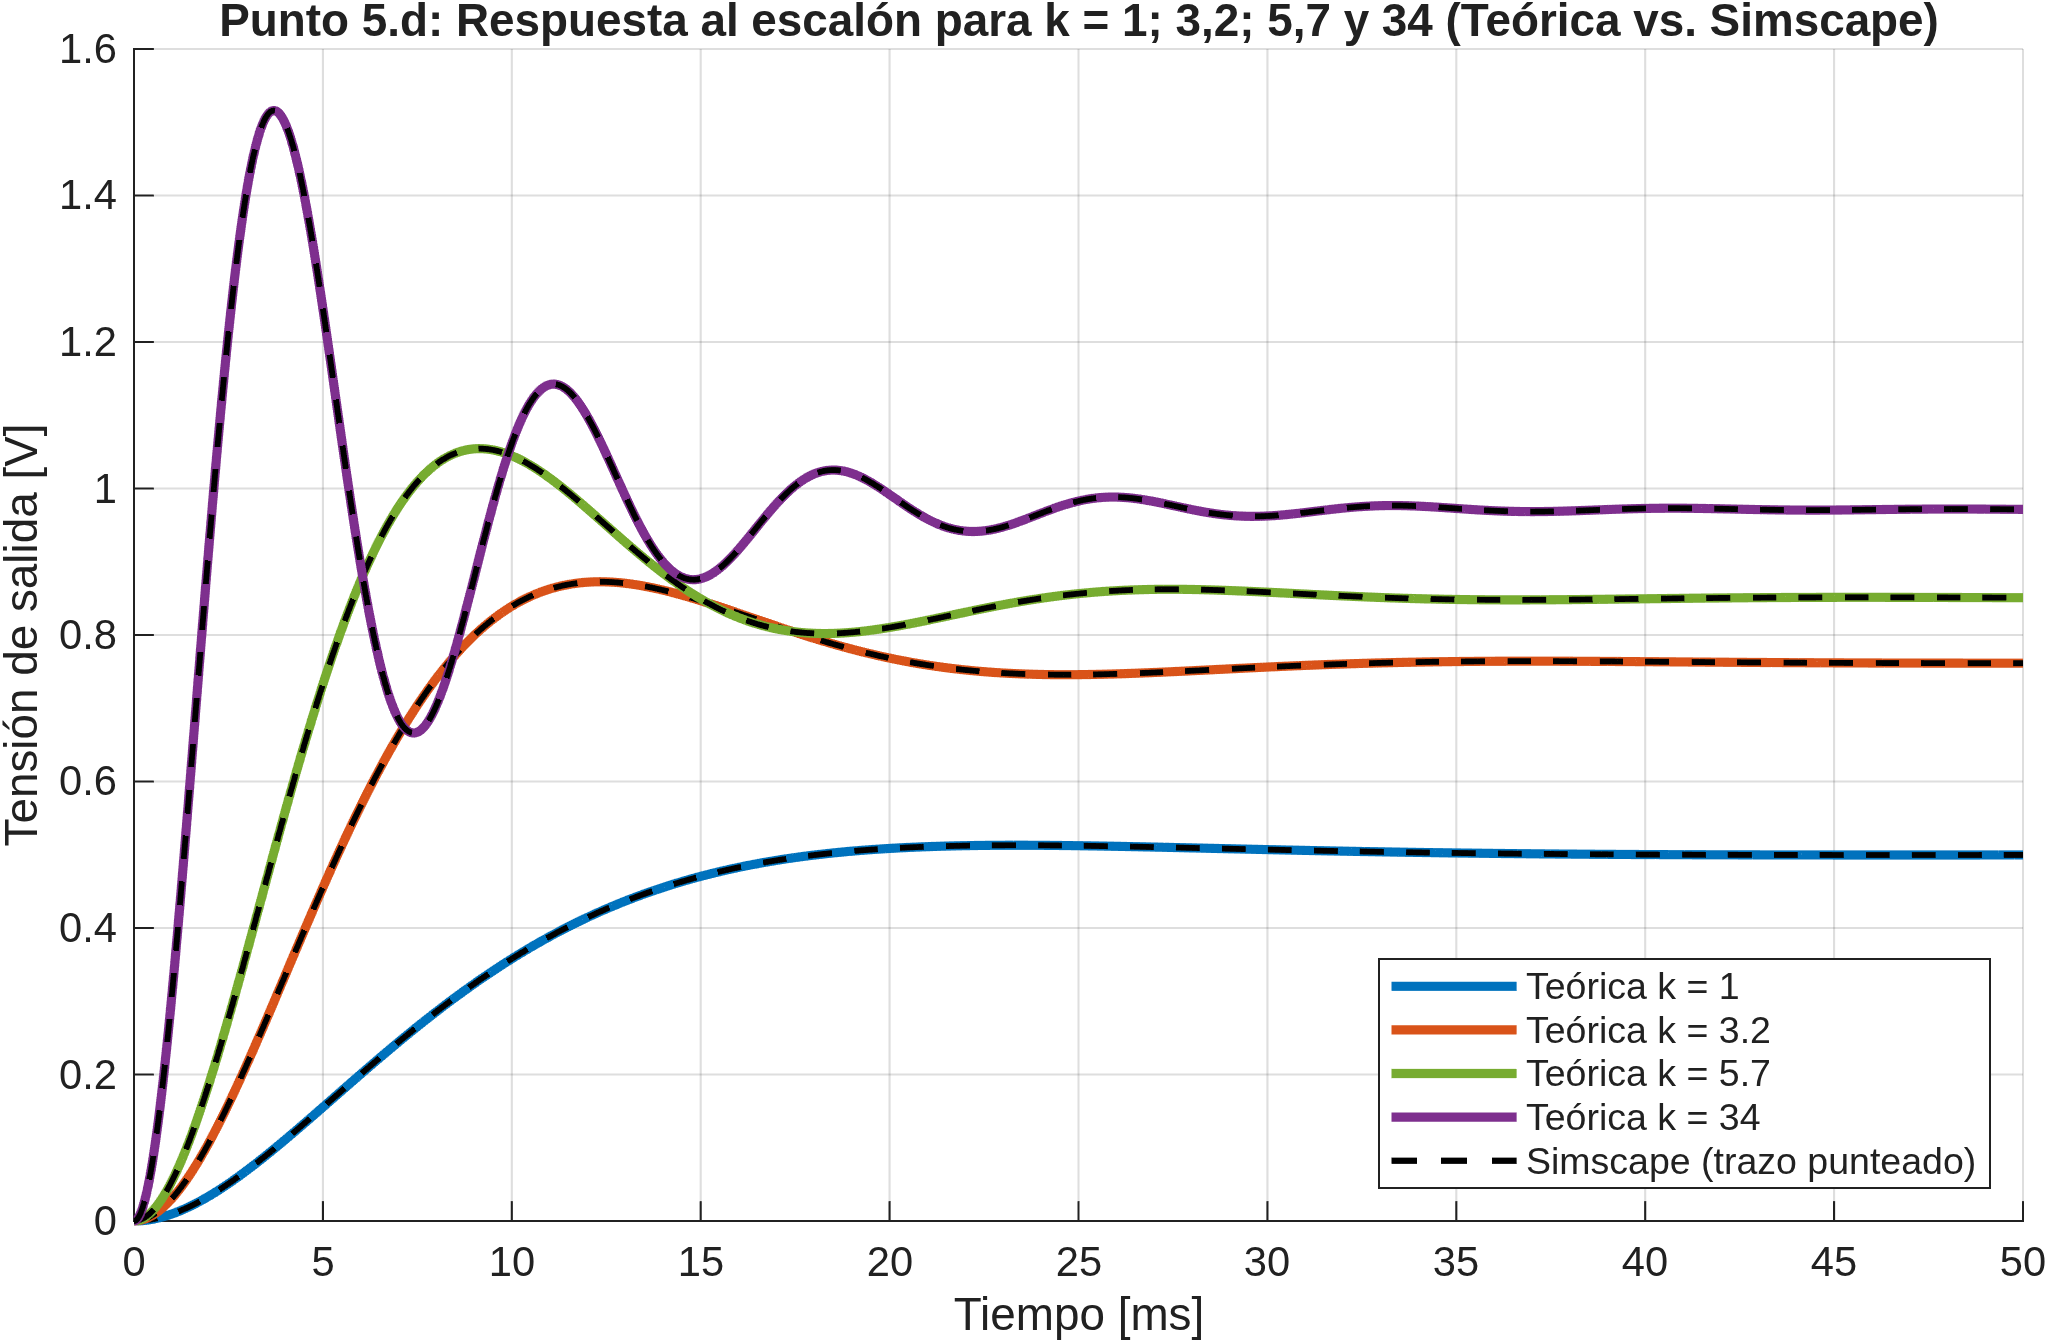
\includegraphics[width=0.82\textwidth]{figuras/punto5d_barrido_k.png}
    \caption{Respuesta al escalón de $1\text{ V}$ para $k = 1$; $3,2$; $5,7$ y $34$: modelo teórico $\text{Sys}_f(s)$ (trazo continuo) vs. Simscape con op-amps ideales (trazo punteado).}
    \label{fig:punto5d}
\end{figure}

\begin{table}[H]
    \centering
    \small
    \begin{tabular}{c c c c c c c c c c}
        \toprule
        & & \multicolumn{2}{c}{\textbf{PO [\%]}} & \multicolumn{2}{c}{\textbf{$T_p$ [s]}} & \multicolumn{2}{c}{\textbf{$T_s$ [s]}} & \multicolumn{2}{c}{\textbf{$y(\infty)$ / $e_{ss}$ [V]}} \\
        \cmidrule(lr){3-4} \cmidrule(lr){5-6} \cmidrule(lr){7-8} \cmidrule(lr){9-10}
        \textbf{$k$} & \textbf{$R_7 / R_9$} & \textbf{Teór.} & \textbf{Sim.} & \textbf{Teór.} & \textbf{Sim.} & \textbf{$4/(\xi\omega_n)$} & \textbf{Sim.} & \textbf{Teór.} & \textbf{Sim.} \\
        \midrule
        $1$   & $0\,\Omega$ / $\infty$            & $2,59$  & $2,65$  & $0,0234$ & $0,0234$ & $0,0256$ & $0,0277$ & $0,5000\,/\,0,5000$ & $0,4997\,/\,0,5003$ \\
        $3,2$ & $2,2\text{ k}\Omega\,/\,1\text{ k}\Omega$ & $14,54$ & $14,59$ & $0,0123$ & $0,0123$ & $0,0256$ & $0,0256$ & $0,7619\,/\,0,2381$ & $0,7616\,/\,0,2384$ \\
        $5,7$ & $4,7\text{ k}\Omega\,/\,1\text{ k}\Omega$ & $23,94$ & $23,91$ & $0,0091$ & $0,0091$ & $0,0256$ & $0,0223$ & $0,8507\,/\,0,1493$ & $0,8509\,/\,0,1491$ \\
        $34$  & $33\text{ k}\Omega\,/\,1\text{ k}\Omega$  & $56,05$ & $56,04$ & $0,0037$ & $0,0037$ & $0,0256$ & $0,0233$ & $0,9714\,/\,0,0286$ & $0,9715\,/\,0,0285$ \\
        \bottomrule
    \end{tabular}
    \caption{Comparación entre parámetros teóricos y medidos sobre la simulación en Simscape para los cuatro valores de $k$.}
    \label{tab:punto5d}
\end{table}

Las leves diferencias en $T_s$ se deben a que la columna teórica reporta la aproximación de envolvente $T_s \approx 4/(\xi\omega_n) = 25,6\text{ ms}$, mientras que la simulación mide el instante exacto en que la curva ingresa por última vez a la banda del $\pm 2\%$.

\section{Circuito con amplificadores operacionales no ideales (TL081)}

\subsection{Comparación en régimen lineal ($k = 11$ y $k = 34$, escalón de $1\text{ V}$)}
Se reemplazaron los tres amplificadores operacionales ideales por el modelo con limitaciones del TL081 alimentado con $\pm 10\text{ V}$ según los datos del Anexo (ganancia de lazo abierto $A = 2 \times 10^5$, resistencia de entrada $R_{\text{in}} = 10^{12}\,\Omega$, resistencia de salida $R_{\text{out}} = 0\,\Omega$ y límites de excursión de tensión de salida $V_{\min} = -8,5\text{ V}$ y $V_{\max} = +8,5\text{ V}$).

En la Fig. \ref{fig:punto6a} y en la Tabla \ref{tab:punto6a} se comparan las respuestas frente a un escalón de $1\text{ V}$ para $k = 11$ ($R_7 = 10\text{ k}\Omega$, $R_9 = 1\text{ k}\Omega$) y $k = 34$ ($R_7 = 33\text{ k}\Omega$, $R_9 = 1\text{ k}\Omega$) entre el modelo ideal y el modelo con TL081.

\begin{figure}[H]
    \centering
    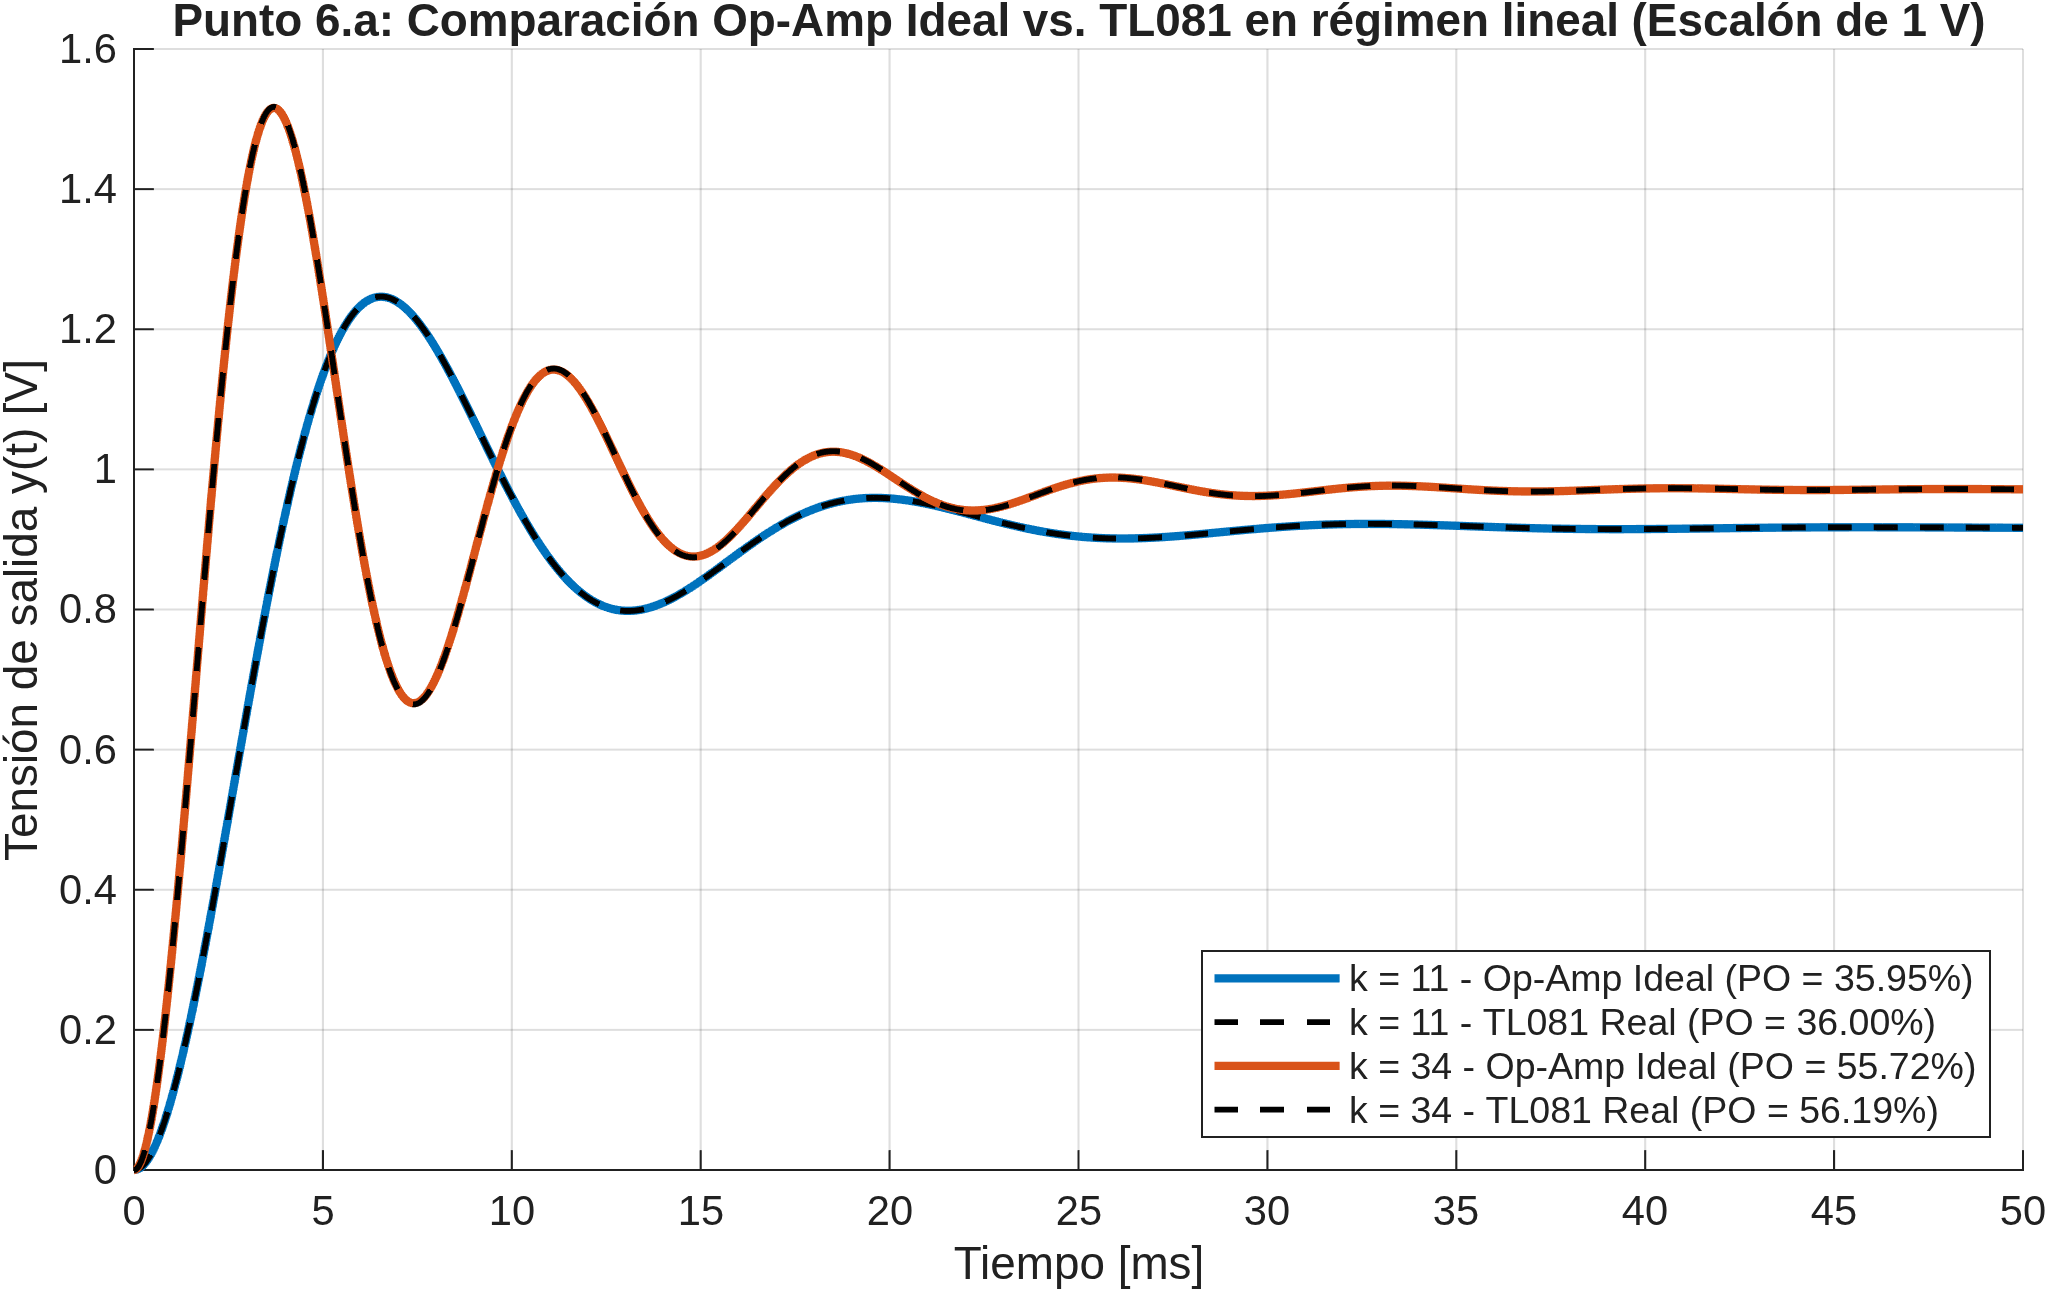
\includegraphics[width=0.78\textwidth]{figuras/punto6a_comparacion.png}
    \caption{Comparación entre op-amps ideales y TL081 en régimen lineal ($1\text{ V}$) para $k = 11$ y $k = 34$.}
    \label{fig:punto6a}
\end{figure}

\begin{table}[H]
    \centering
    \small
    \setlength{\tabcolsep}{4pt}
    \begin{tabular}{c c c c c c c c c}
        \toprule
        \textbf{$k$} & \textbf{Modelo} & \textbf{$PO$ [\%]} & \textbf{$T_p$ [ms]} & \textbf{$T_s$ [ms]} & \textbf{$t_r$ [ms]} & \textbf{$y_{\text{pico}}$ [V]} & \textbf{$y(\infty)$ [V]} & \textbf{Error máx. vs. Ideal} \\
        \midrule
        $11$ & Ideal & $35,97$ & $6,5$ & $22,2$ & $2,6$ & $1,2464$ & $0,9167$ & --- \\
        $11$ & TL081 & $35,99$ & $6,5$ & $22,2$ & $2,6$ & $1,2466$ & $0,9167$ & $0,21\text{ mV}$ \\
        \midrule
        $34$ & Ideal & $56,05$ & $3,7$ & $23,3$ & $1,4$ & $1,5159$ & $0,9714$ & --- \\
        $34$ & TL081 & $56,20$ & $3,7$ & $23,3$ & $1,4$ & $1,5174$ & $0,9714$ & $1,69\text{ mV}$ \\
        \bottomrule
    \end{tabular}
    \caption{Parámetros de la respuesta temporal al escalón unitario: op-amp ideal vs. TL081.}
    \label{tab:punto6a}
\end{table}

Para un escalón de $1\text{ V}$, la tensión de salida alcanza como máximo $1,25\text{ V}$ ($k = 11$) y $1,52\text{ V}$ ($k = 34$). Como en ambos casos las tensiones se mantienen muy por debajo de los límites de saturación de $\pm 8,5\text{ V}$, los operacionales trabajan siempre en su zona lineal. Dado que el TL081 tiene una ganancia de lazo abierto muy elevada ($A = 2 \times 10^5$) y una impedancia de entrada muy alta ($10^{12}\,\Omega$), su comportamiento en zona lineal es prácticamente idéntico al del operacional ideal (con diferencias menores a $2\text{ mV}$).

\subsection{Amplitud de escalón para el inicio del recorte ($k = 34$)}
Para $k = 34$, con una ganancia estática $y(\infty) = \frac{34}{35} \approx 0,9714\text{ V}$ y un sobrepaso $PO = 56,05\%$, el valor pico por cada voltio de escalón de entrada es:
\begin{equation}
    y_{\text{pico, 1V}} = \frac{34}{35}\left(1 + \frac{PO}{100}\right) = 1,5159\text{ V/V} \approx 1,52\text{ V/V}
\end{equation}
Como el TL081 alimentado con $\pm 10\text{ V}$ satura su salida en $V_{\max} = 8,5\text{ V}$, la amplitud del escalón de entrada a partir de la cual la salida de $U_{2A}$ alcanza el recorte es:
\begin{equation}
    A_{\text{recorte}} = \frac{V_{\max}}{y_{\text{pico, 1V}}} = \frac{8,5\text{ V}}{1,52\text{ V/V}} \approx 5,59\text{ V}
\end{equation}

\subsection{Simulación con escalones de $5\text{ V}$ y $7\text{ V}$ ($k = 34$)}
Se simuló el circuito con TL081 frente a escalones de $5\text{ V}$ y $7\text{ V}$, superponiendo los resultados con la respuesta de $\text{Sys}_f(s)$ en la Fig. \ref{fig:punto6c} y resumiendo las medidas en la Tabla \ref{tab:punto6c}.

\begin{figure}[H]
    \centering
    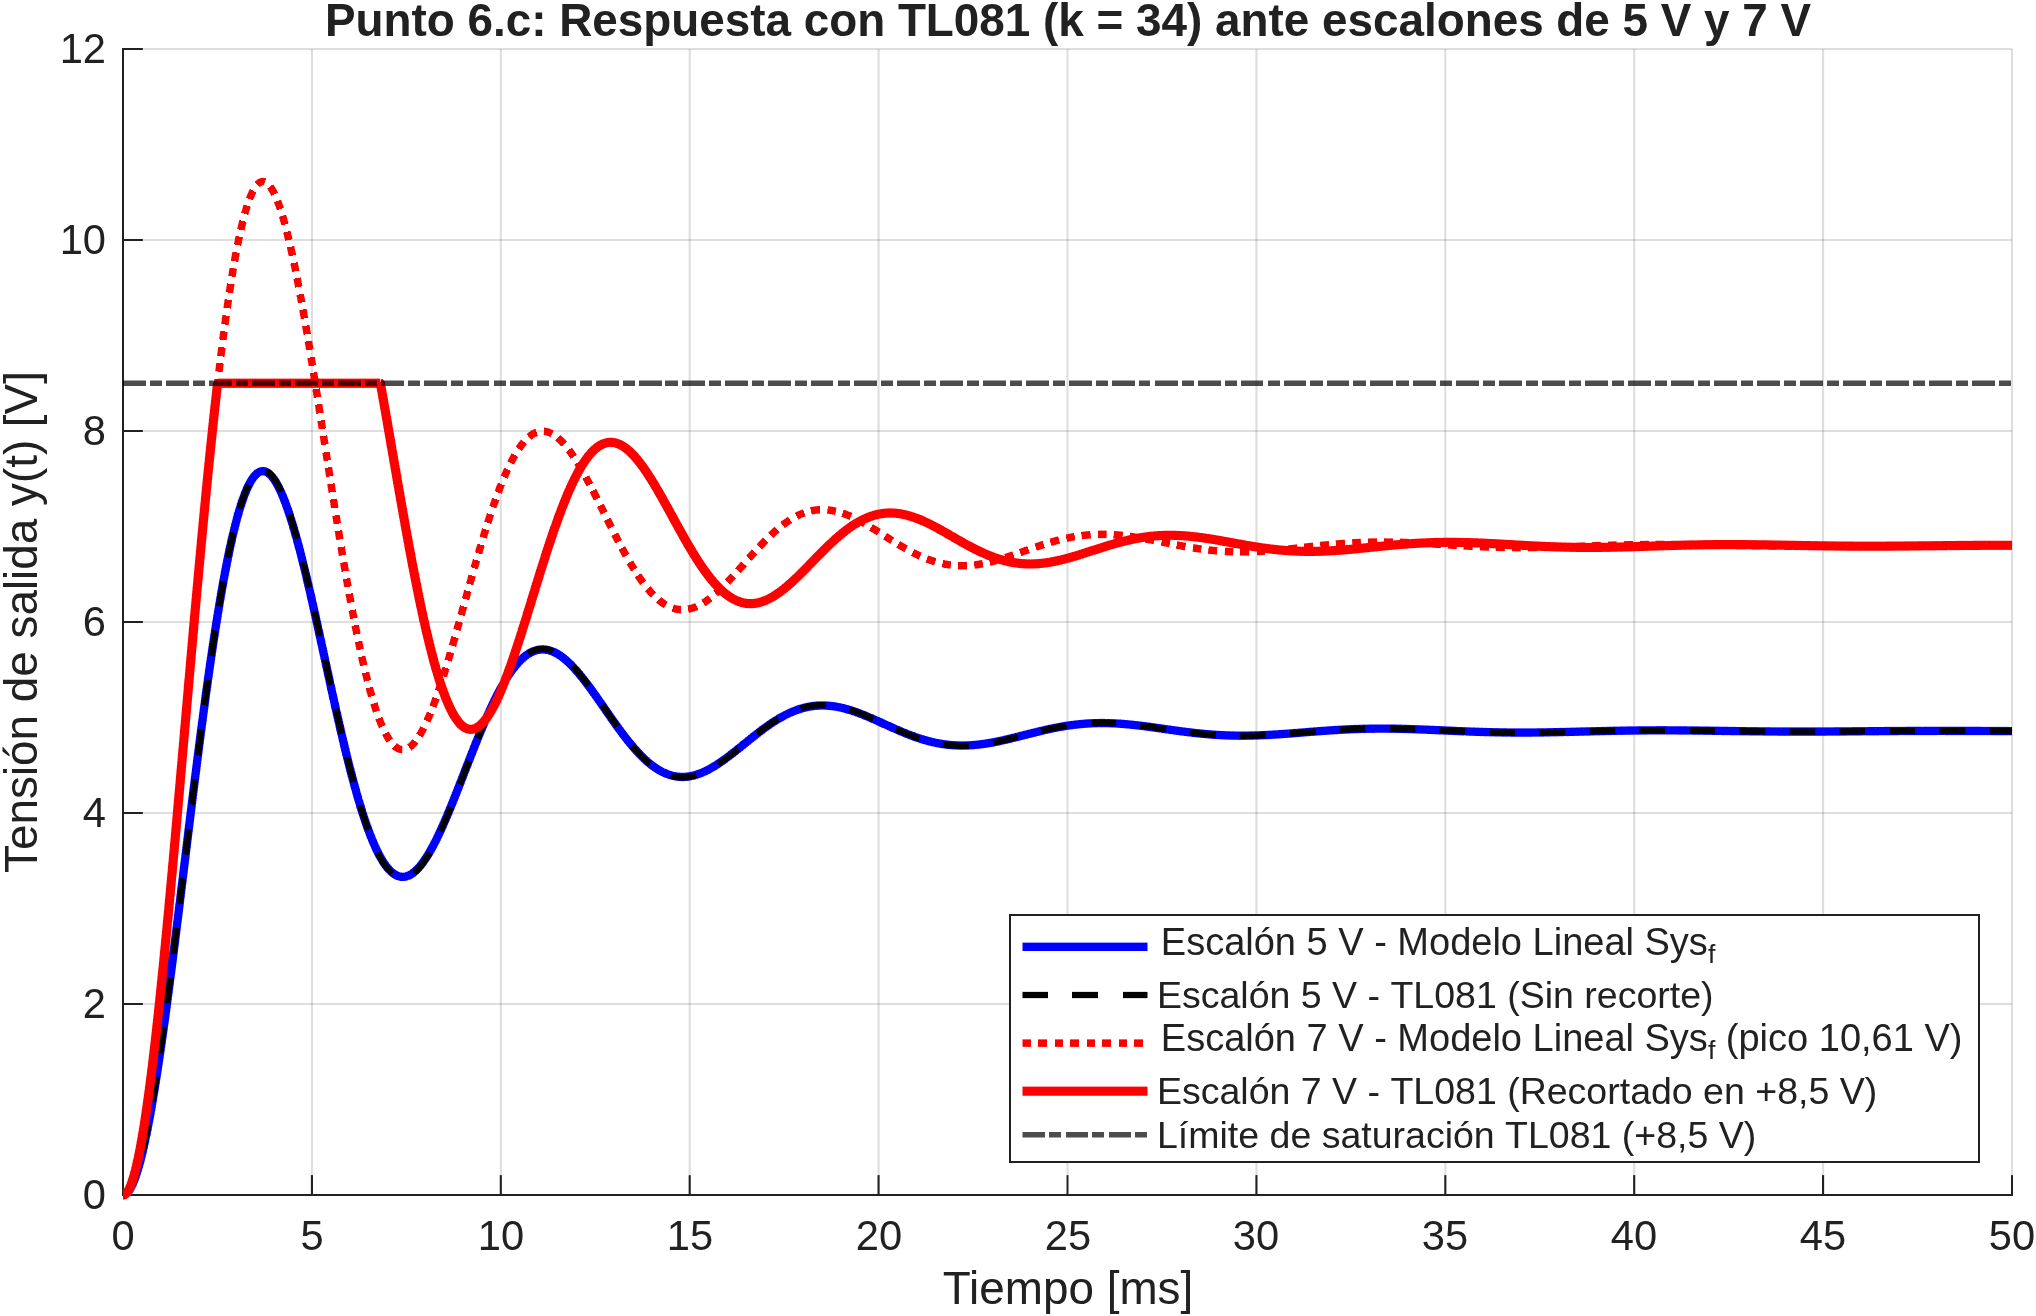
\includegraphics[width=0.78\textwidth]{figuras/punto6c_saturacion.png}
    \caption{Respuesta con TL081 ($k = 34$) ante escalones de $5\text{ V}$ (lineal) y $7\text{ V}$ (saturación en $8,5\text{ V}$).}
    \label{fig:punto6c}
\end{figure}

\begin{table}[H]
    \centering
    \small
    \begin{tabular}{l c c c c c c}
        \toprule
        \textbf{Entrada} & \textbf{Modelo} & \textbf{$y_{\text{pico}}$ [V]} & \textbf{$PO$ [\%]} & \textbf{$T_p$ [ms]} & \textbf{$T_s$ [ms]} & \textbf{$y(\infty)$ [V]} \\
        \midrule
        Escalón $5\text{ V}$ & $\text{Sys}_f$ lineal & $7,58$ & $56,05$ & $3,7$ & $23,3$ & $4,8571$ \\
        Escalón $5\text{ V}$ & TL081 (Sim.)          & $7,59$ & $56,20$ & $3,7$ & $23,3$ & $4,8571$ \\
        \midrule
        Escalón $7\text{ V}$ & $\text{Sys}_f$ lineal & $10,61$ & $56,05$ & $3,7$ & $23,3$ & $6,8000$ \\
        Escalón $7\text{ V}$ & TL081 (Sim.)          & $8,50$ & $25,00$ & $2,5^*$ & $25,0$ & $6,8000$ \\
        \bottomrule
    \end{tabular}
    \caption{Comparación entre el modelo lineal y el circuito con TL081 ante escalones de $5\text{ V}$ y $7\text{ V}$. ($^*$Instante en el que alcanza el límite de $8,50\text{ V}$).}
    \label{tab:punto6c}
\end{table}

\begin{itemize}
    \item \textbf{Escalón de $5\text{ V}$ ($A < 5,59\text{ V}$):} La salida alcanza un pico de $7,59\text{ V} < 8,5\text{ V}$. Como no supera el límite del operacional, el circuito se mantiene en zona lineal y la respuesta es simplemente $5$ veces la del escalón unitario, coincidiendo con $\text{Sys}_f(s)$.
    \item \textbf{Escalón de $7\text{ V}$ ($A > 5,59\text{ V}$) y por qué $\text{Sys}_f(s)$ deja de describir al circuito:} Una función de transferencia solo es válida para sistemas lineales (donde vale la proporcionalidad). Para $7\text{ V}$, el modelo lineal predice un pico de $10,61\text{ V}$, pero el operacional $U_{2A}$ satura y recorta la salida en $+8,50\text{ V}$. Este tope físico es un efecto no lineal que la función de transferencia $\text{Sys}_f(s)$ no contempla, reduciendo el sobrepaso real al $25\%$ y modificando el transitorio hasta que la tensión baja de $8,5\text{ V}$ y el circuito converge al valor estacionario $y(\infty) = 6,80\text{ V}$ (que sí está en zona lineal).
\end{itemize}

\section{Sensibilidad a las tolerancias de componentes}

\subsection{Identificación y justificación analítica de los casos extremos ($k = 11$)}
Considerando resistores al $\pm 5\%$ y capacitores al $\pm 10\%$, el sobrepaso $PO = 100\,e^{-\pi\xi/\sqrt{1-\xi^2}}$ aumenta a medida que disminuye el factor de amortiguamiento $\xi$, por lo que el mayor sobrepaso ocurre con $\xi$ mínimo y el menor con $\xi$ máximo. A partir de las expresiones obtenidas en el Punto 1 ($\tau_1 = R_1 C_1$, $\tau_2 = R_2 C_2$ y $k = 1 + R_7/R_9$):
\begin{equation}
    \omega_n = \sqrt{\frac{1+k}{\tau_1 \tau_2}}, \qquad \xi = \frac{\tau_1 + \tau_2}{2\sqrt{\tau_1 \tau_2 (1+k)}}
\end{equation}

Analizando cómo influyen los componentes sobre $\xi$:
\begin{enumerate}
    \item \textbf{Ganancia $k = 1 + R_7/R_9$:} Como $(1+k)$ está dividiendo dentro de la raíz, $\xi$ disminuye cuando $k$ aumenta. Por lo tanto, se tiene menor $\xi$ (mayor $PO$) cuando $k$ es máximo ($R_7$ en $+5\%$ y $R_9$ en $-5\%$, dando $k_{ef} = 12,053$), y mayor $\xi$ (menor $PO$) cuando $k$ es mínimo ($R_7$ en $-5\%$ y $R_9$ en $+5\%$, dando $k_{ef} = 10,048$).
    \item \textbf{Constantes de tiempo $\tau_1$ y $\tau_2$:} El cociente $\frac{\tau_1 + \tau_2}{\sqrt{\tau_1 \tau_2}}$ es mínimo cuando $\tau_1$ y $\tau_2$ se acercan entre sí, y crece cuando se alejan. Como nominalmente $\tau_1 = 10\text{ ms}$ es mayor que $\tau_2 = 4,7\text{ ms}$:
    \begin{itemize}
        \item Para menor $\xi$ (mayor $PO$), hay que acercar ambas constantes de tiempo: $\tau_1$ al mínimo ($R_1 -5\%$, $C_1 -10\%$) y $\tau_2$ al máximo ($R_2 +5\%$, $C_2 +10\%$).
        \item Para mayor $\xi$ (menor $PO$), hay que alejarlas: $\tau_1$ al máximo ($R_1 +5\%$, $C_1 +10\%$) y $\tau_2$ al mínimo ($R_2 -5\%$, $C_2 -10\%$).
    \end{itemize}
\end{enumerate}

En la Tabla \ref{tab:punto7a} se resumen las combinaciones de componentes y los parámetros resultantes.

\begin{table}[H]
    \centering
    \footnotesize
    \setlength{\tabcolsep}{2.8pt}
    \begin{tabular}{l c c c c c c c c c c}
        \toprule
        \textbf{Condición} & \textbf{$R_1$ [k$\Omega$]} & \textbf{$C_1$ [nF]} & \textbf{$R_2$ [k$\Omega$]} & \textbf{$C_2$ [nF]} & \textbf{$R_7$ [k$\Omega$]} & \textbf{$R_9$ [k$\Omega$]} & \textbf{$\tau_1$ [ms]} & \textbf{$\tau_2$ [ms]} & \textbf{$k_{ef}$} & \textbf{$\xi$} \\
        \midrule
        Mayor sobrepaso ($PO_{\max}$) & $95,0$ & $90$ & $49,35$ & $110$ & $10,5$ & $0,95$ & $8,550$ & $5,429$ & $12,053$ & $0,2840$ \\
        Caso nominal & $100,0$ & $100$ & $47,00$ & $100$ & $10,0$ & $1,00$ & $10,000$ & $4,700$ & $11,000$ & $0,3095$ \\
        Menor sobrepaso ($PO_{\min}$) & $105,0$ & $110$ & $44,65$ & $90$ & $9,5$ & $1,05$ & $11,550$ & $4,019$ & $10,048$ & $0,3438$ \\
        \bottomrule
    \end{tabular}
    \caption{Combinaciones extremas de componentes pasivos y parámetros resultantes ($k = 11$).}
    \label{tab:punto7a}
\end{table}

\subsection{Simulación de los casos extremos en Simscape}
En la Fig. \ref{fig:punto7b} se superponen las respuestas al escalón unitario obtenidas en Simscape para los dos casos extremos y el caso nominal, y en la Tabla \ref{tab:punto7b} se informan los parámetros medidos.

\begin{figure}[H]
    \centering
    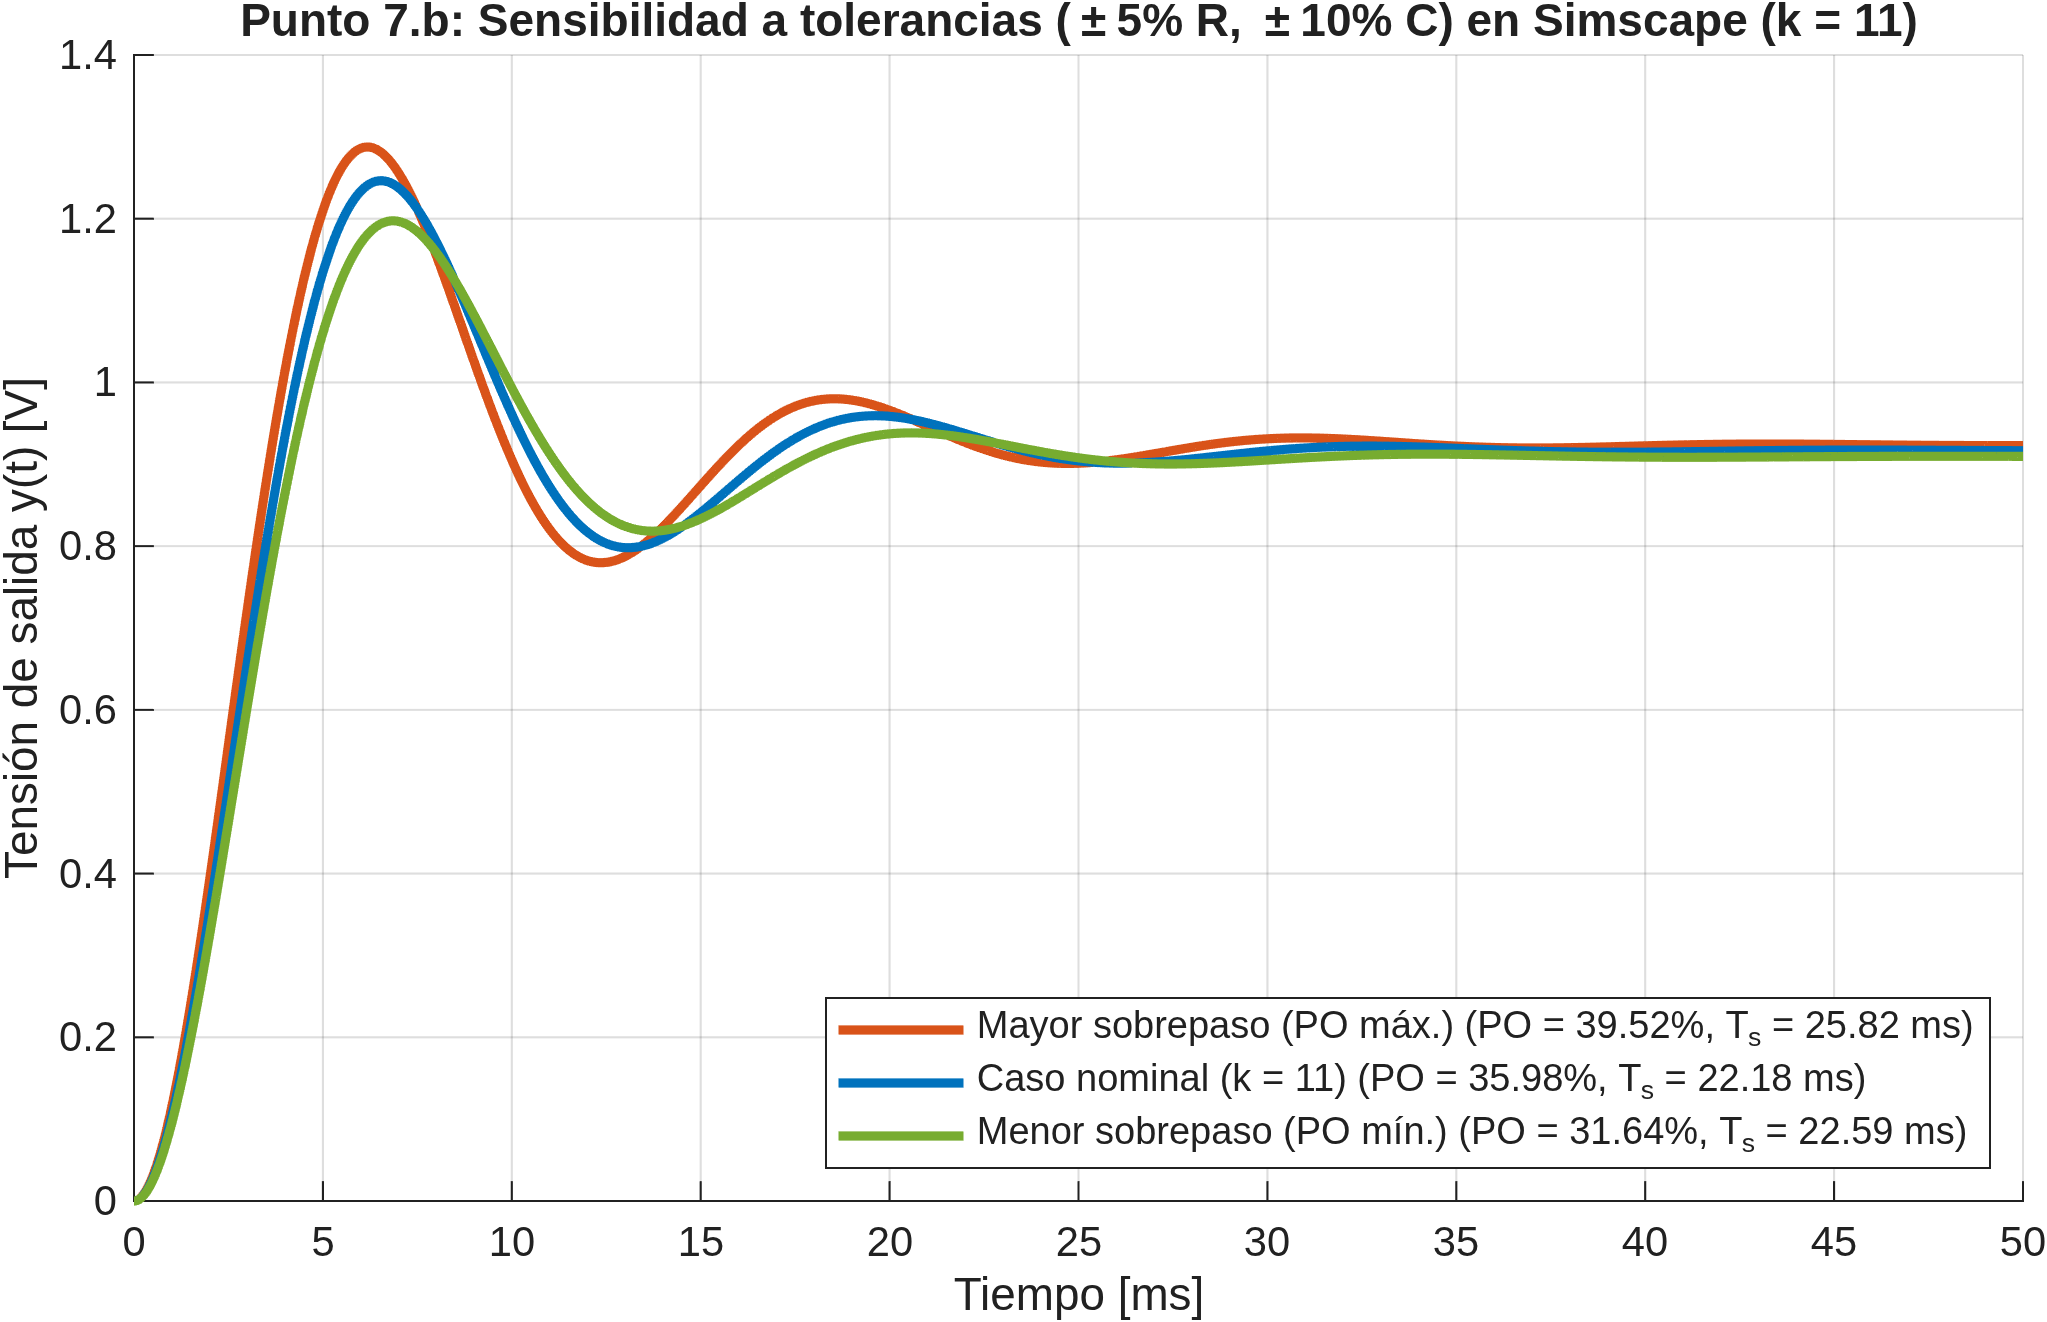
\includegraphics[width=0.78\textwidth]{figuras/punto7b_tolerancias.png}
    \caption{Simulación en Simscape de los casos extremos de tolerancia pasiva junto con el caso nominal ($k = 11$).}
    \label{fig:punto7b}
\end{figure}

\begin{table}[H]
    \centering
    \small
    \setlength{\tabcolsep}{5pt}
    \begin{tabular}{l c c c c c c c}
        \toprule
        \textbf{Condición} & \textbf{$\omega_n$ [rad/s]} & \textbf{$\xi$} & \textbf{$PO$ [\%]} & \textbf{$T_p$ [ms]} & \textbf{$T_s$ [ms]} & \textbf{$y(\infty)$ [V]} & \textbf{$e_{ss}$ [V]} \\
        \midrule
        Menor sobrepaso ($PO_{\min}$) & $487,9$ & $0,3438$ & $31,66$ & $6,9$ & $22,6$ & $0,9095$ & $0,0905$ \\
        Caso nominal ($k = 11$)       & $505,3$ & $0,3095$ & $35,97$ & $6,5$ & $22,2$ & $0,9167$ & $0,0833$ \\
        Mayor sobrepaso ($PO_{\max}$) & $530,3$ & $0,2840$ & $39,44$ & $6,2$ & $25,9$ & $0,9234$ & $0,0766$ \\
        \bottomrule
    \end{tabular}
    \caption{Resultados de simulación en Simscape para los casos extremos de tolerancia pasiva ($k = 11$).}
    \label{tab:punto7b}
\end{table}

\textbf{Rangos de variación de $PO$ y $T_s$:}
\begin{itemize}
    \item \textbf{Sobrepaso porcentual ($PO$):} Varía entre $31,66\%$ y $39,44\%$ (un rango total de $\Delta PO = 7,78$ puntos porcentuales).
    \item \textbf{Tiempo de establecimiento ($T_s$):} Según la envolvente teórica $4/(\xi\omega_n)$, el tiempo disminuye de $26,6\text{ ms}$ ($PO_{\max}$) a $25,6\text{ ms}$ (nominal) y $23,9\text{ ms}$ ($PO_{\min}$). Medido sobre la simulación con el criterio exacto del $\pm 2\%$, varía entre $22,2\text{ ms}$ y $25,9\text{ ms}$ ($\Delta T_s = 3,7\text{ ms}$), ya que en el caso nominal y en el de $PO_{\min}$ el valle siguiente queda apenas dentro de la banda del $2\%$ y el cruce se define en el ciclo previo (donde $PO_{\min}$ cruza $0,4\text{ ms}$ después por tener menor $\omega_n$).
\end{itemize}

\subsection{Comparación entre el efecto de las tolerancias y el op-amp real}
En la Tabla \ref{tab:punto7c} se compara la variación de $PO$ y $T_s$ producida por las tolerancias de los componentes (Punto 7.b) con la producida al reemplazar los op-amps ideales por el TL081 en régimen lineal (Punto 6.a, $k = 11$).

\begin{table}[H]
    \centering
    \small
    \begin{tabular}{l c c c}
        \toprule
        \textbf{Efecto considerado ($k = 11$)} & \textbf{Rango de $PO$ [\%]} & \textbf{$|\Delta PO|$ [\%]} & \textbf{$|\Delta T_s|$ [ms]} \\
        \midrule
        Tolerancias de componentes ($\pm 5\%$ en $R$, $\pm 10\%$ en $C$) & $31,66$ a $39,44$ & $7,78$ & $3,7$ \\
        Reemplazo por op-amp TL081 en zona lineal (Punto 6.a)            & $35,97$ a $35,99$ & $0,02$ & $< 0,1$ \\
        \bottomrule
    \end{tabular}
    \caption{Comparación entre el efecto de las tolerancias y el reemplazo por el TL081 en régimen lineal.}
    \label{tab:punto7c}
\end{table}

\textbf{Efecto dominante:} Domina claramente la variación por las tolerancias de los componentes pasivos ($\Delta PO = 7,78\%$ y $\Delta T_s = 3,7\text{ ms}$), mientras que el cambio por usar el TL081 en régimen lineal es prácticamente despreciable ($\Delta PO = 0,02\%$ y $\Delta T_s < 0,1\text{ ms}$).

\end{document}
